\documentclass[runningheads]{llncs}

\usepackage[T1]{fontenc}

\usepackage{graphicx} % Required for inserting images
\usepackage{graphics} % for pdf, bitmapped graphics files
\usepackage{svg} % for svgs
\usepackage{epsfig} % for postscript graphics files
%\usepackage{mathptmx} % assumes new font selection scheme installed
%\usepackage{times} % assumes new font selection scheme installed
\usepackage[ruled,vlined]{algorithm2e}
\usepackage{amsmath}
\usepackage{amsthm}
\usepackage{amssymb}  % assumes amsmath package installed

%\usepackage{type1cm}
%\usepackage{url}
\usepackage{hyperref}
\hypersetup{
    colorlinks=true,
    linkcolor=blue,
    filecolor=magenta,      
    urlcolor=blue,
    citecolor=black,
    pdftitle={Overleaf Example},
    pdfpagemode=FullScreen,
    }
\urlstyle{same}
\usepackage{tikz}
\usepackage{ifthen}
\usetikzlibrary {arrows.meta}
\usetikzlibrary{positioning}
%\usepackage{bm}

\SetKwComment{Comment}{/* }{ */}
\SetKw{not}{not}
\SetKw{and}{and}

\setlength{\textfloatsep}{10pt plus 2pt minus 4pt}
\setlength{\floatsep}{8pt plus 2pt minus 2pt}
\setlength{\intextsep}{10pt plus 2pt minus 2pt}



% \IEEEoverridecommandlockouts
% \overrideIEEEmargins
% \pdfminorversion=4

\title{A Scalable Strategy for Resource-Constrained Shape-Changing Robots in Dense Swarms}

\titlerunning{Strategy for Shape-Changing Robots}

\author{Alexandra Nilles\inst{1,3}, Henry Boekhoff\inst{3}, Heather Jin Hee Kim\inst{2}, Julian Prieto\inst{2}, Elizabeth Garner\inst{1} and Kirstin Petersen\inst{1}}

\authorrunning{A. Nilles et al.}

\institute{School of Electrical and Computer Engineering, Cornell University, Ithaca NY, USA \and Sibley School of Mechanical and Aerospace Engineering, Cornell University, Ithaca NY, USA
\and Department of Computer Science, Western Washington University, Bellingham WA, USA}


\begin{document}


\maketitle


\begin{abstract}
Local geometric interactions play an important role in the collective coordination of artificial and biological agents, especially in the case of distributed protocols. In robotic systems, these local interactions are implemented primarily through explicit sensing, state estimation, and communication between robots. We ask instead how mechanical interactions and embodied computation can be leveraged to affect collective coordination. In this paper, we  propose minimalist algorithms for swarms of shape-changing robots. Each robot has random or ``wild'' motion, local contact sensing, and minimal memory and computation. To support analysis of our proposed algorithm, we introduce a shape-shifting robotic platform for studies of ``morphological coordination,'' and a corresponding simulator. Our findings, in hardware and simulation, indicate effective strategies for controlling collective ``shape allocation'' using a single global input parameter. We extend results connecting Poisson point processes to statistical properties of dense robot swarms, considering the case of the binary shape-change decision problem. We perform exploratory Monte Carlo analysis of system sensitivity to local density, algorithm timer thresholds. Interestingly, we find that shape-change between convex and oblong shapes does not significantly affect the clustering behavior of the robot collective in free space, but appears to be more significant in confined spaces when the collective is driven by uniform global controls or forces. Our results are especially interesting in the context of design of micro/nano-robotic systems (``smart matter''), and the implications for the design of these systems are discussed.
 
\end{abstract}

\keywords{Multi-Agent Systems, Distributed Robotics, Micro/Nano Robots}

\section{INTRODUCTION}

A key behavior of decentralized, multi-robot systems is the ability to intermittently make contact with other agents to exchange information, especially in consensus-based or cooperative tasks. Multi-robot systems with range-limited wireless communication must assume robots are well-mixed in their environment \cite{edwards2023collaborative} or can perform periodic motion patterns \cite{yu2021resilient} to ensure consensus despite intermittent communication. However, as multi-robot systems scale up in number, we must minimize system energy use, which can easily become dominated by communication systems. As the robotic agents themselves scale down in size, enabled by advances in nano/micro-scale robotic and biohybrid systems \cite{wang2021trends}, traditional wireless communication technologies become impractical for collective coordination. However, the intentional design of direct robot-robot collisions is becoming feasible due to advances in materials and robot design, especially for micro/nano-robots due to the physics at these scales. The ability to at worst tolerate collisions and at best extract information from them is also an active area of development for field robotics in settings where collisions are inevitable due to environment geometry or dynamics, such as navigation through pipes.

Many biological systems, from herds of mammals to bacterial biofilms, use mechanical agent-agent interactions for coordination. This strategy has been used for collective robot density estimation and localization in known environments \cite{mayya2018localization,mayya2019closed}. In this paper, we add the idea that robots can process information and react to stimuli via their morphology. We focus on morphology as the primary actuation, both because shape-changing particles are becoming a practical reality for micro/nano-robots \cite{tanjeem2022shape,tan2023shape} and because this is a novel topic of study where robotic platforms can be used to study the underlying physical phenomenon in active matter systems, similarly to how legged robots have assisted in the direct study of locomotion robophysics \cite{aguilar2016review}. We develop a macro-scale testbed that emulates properties of micro-scale active matter particles, and use this testbed to study the effect of controllable agent morphology on system-level aggregation dynamics. Our contributions in this work include:

\begin{itemize}
\item the development of a decentralized shape-change algorithm based on encounter-rate quorum sensing with minimal memory and no wireless communication;
\item the implementation of macro-scale shape-shifting active particle robots and corresponding simulator; and
\item several results on the analysis of this algorithm and its sensitivity to system parameters.
\end{itemize}



\begin{figure}[t]
\centering
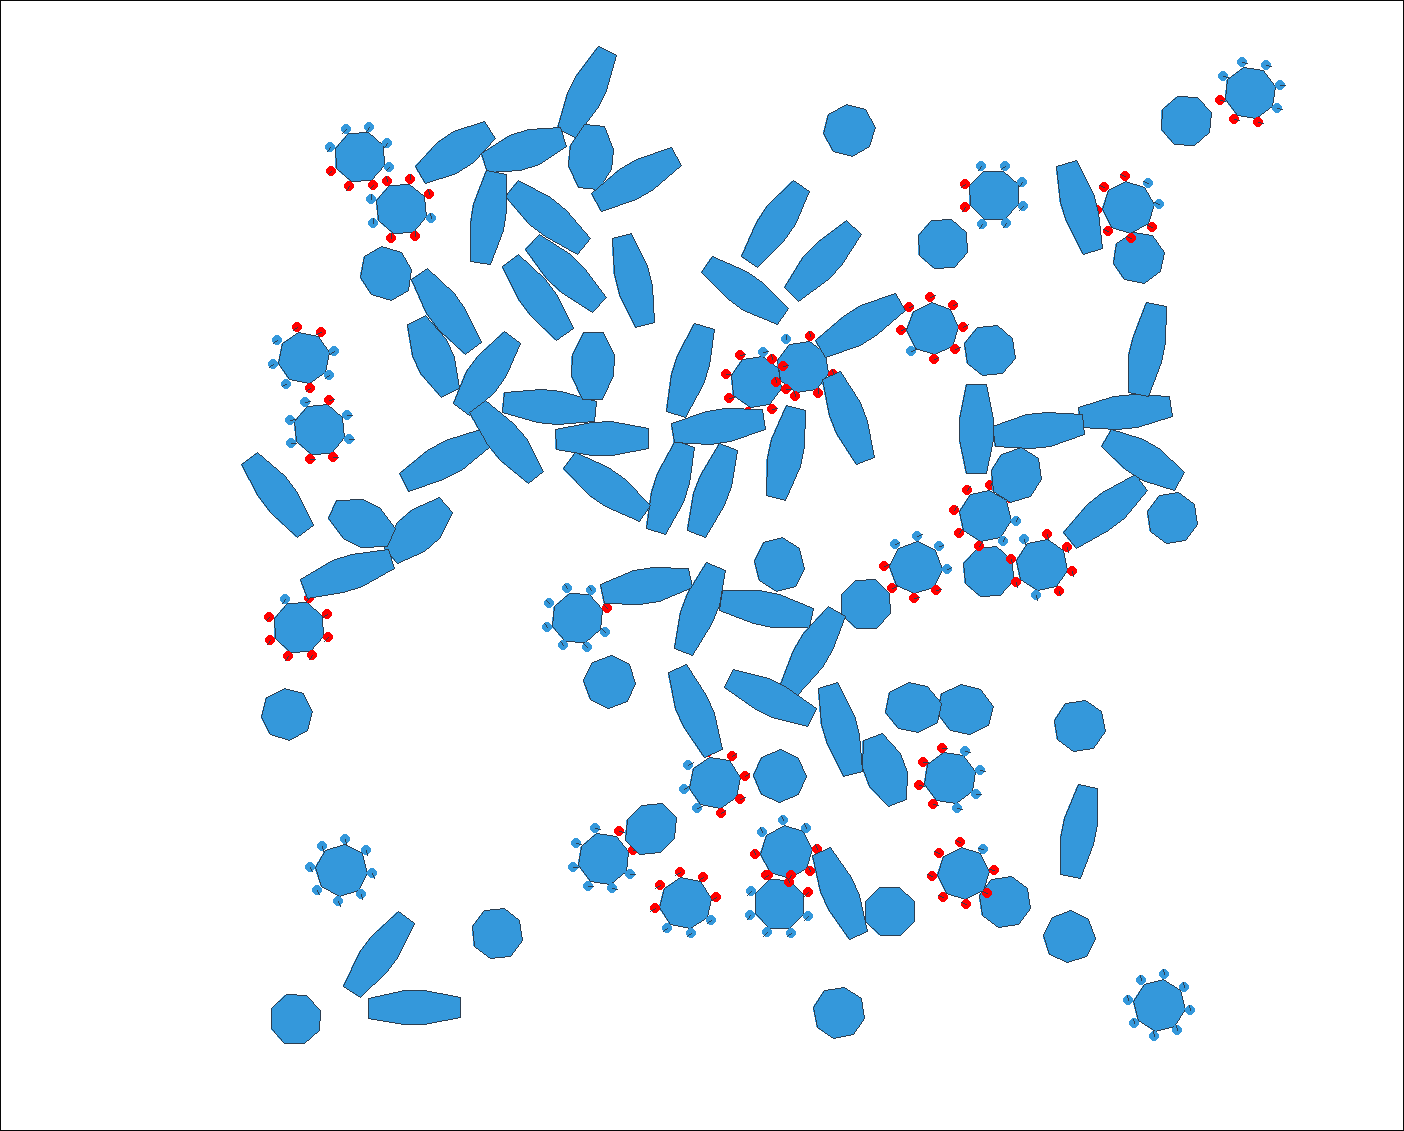
\includegraphics[height=0.45\linewidth, width=.5\linewidth]{figs/simulation_screenshot2.png}\hfill
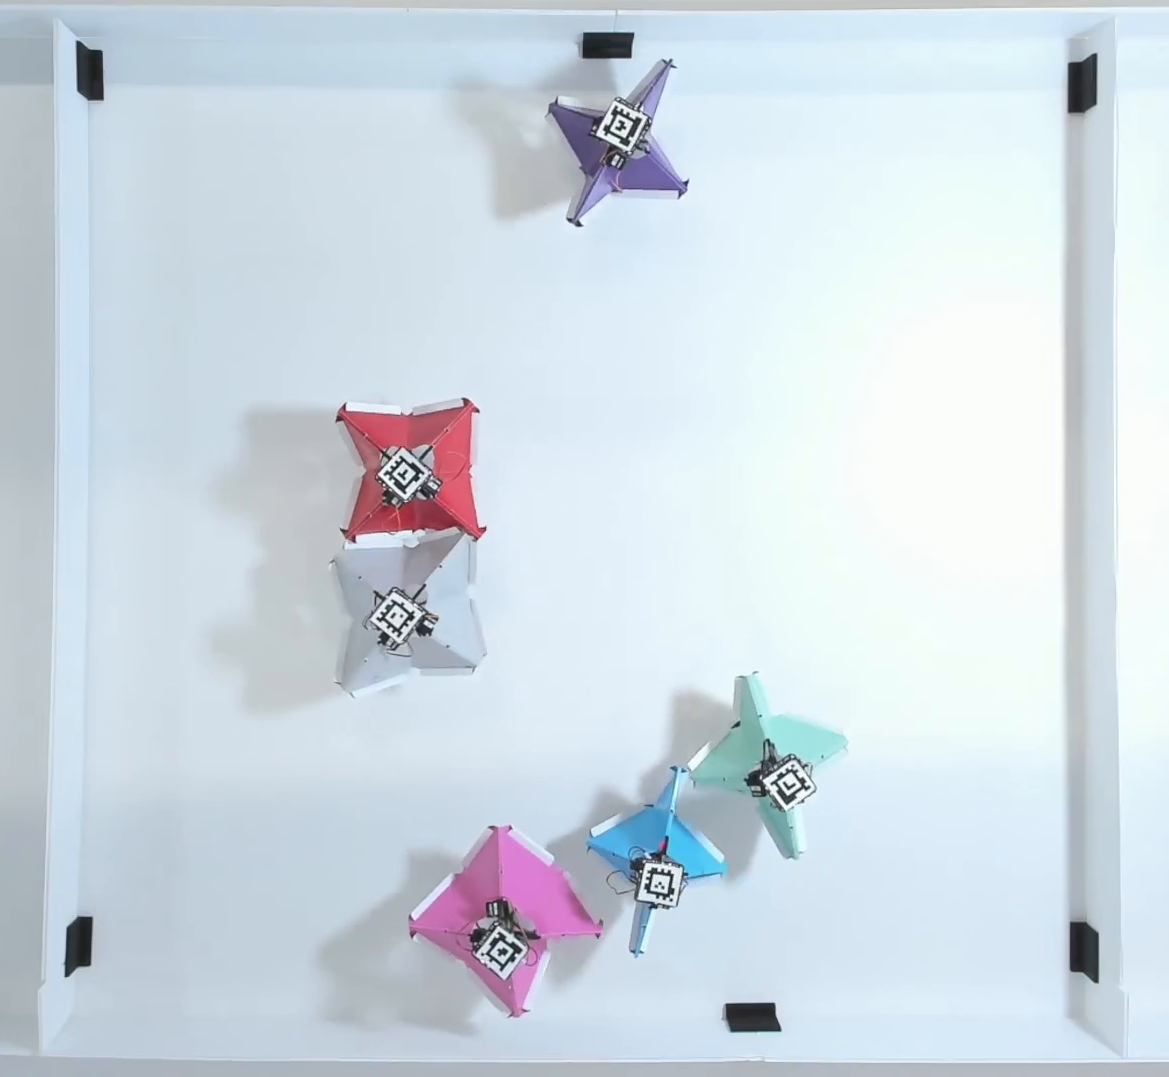
\includegraphics[height=0.45\linewidth]{figs/experiment_capture1.png}
    \caption{(Left) Single frame from PyMunk simulation, showing 100 bots (most oblong, some octagon). Red dots indicate active collisions. (Right) A frame from hardware experimentation, showing six bots (three convex and three nonconvex).}
    \label{fig:sim}
\end{figure}

%We are simultaneously developing a macro-scale testbed that emulates properties of micro-scale active matter particles, as well as directly studying the effect of controllable agent morphology on system-level aggregation dynamics.

\subsection{Related Work}

\subsubsection{Wild Bodies and Synthetic Cells}
\emph{Wild bodies} are a class of agents that in informal terms are guaranteed to eventually explore all of their environment. 
One line of work implements control synthesis for wild body density via environment geometry design and active ``doorways'' \cite{bobadilla2012controlling,gierl2014stochastic}. 
Another line of work considers the construction of low-complexity combinatorial filters for counting wild bodies with single-bit sensor beams \cite{erickson2013counting}. In \cite{pervan2018low} the authors investigate automatic co-design of controllers and sensors for minimalist artificial agents such as synthetic cells . Such approaches give up precise control of individual agents in exchange for probabilistic guarantees on system accuracy.

Synthetic cells often exhibit a combination of controlled and brownian motion, leading to the development of the \emph{active Brownian particle} (ABP) model inspired by biological and artificial agents moving in low-Reynolds-number environments. This model has been the subject of recent study in mechanics and materials science, especially in complex and crowded environments \cite{bechinger2016active} where collectives of ABPs exhibit interesting collective behaviors that may be useful for novel colloidal ``smart'' materials. Another application area of ``synthetic cells" may be bio-medical research, as an alternative to optical tweezers when interacting with biological cells in controlled environments \cite{ivanyi2024optically}, or medical interventions within the human body using swarms of smart particles \cite{xie2025microrobotic}.

When studying wild or stochastic agents that can handle collisions, it is clear that body morphology and ``embodied intelligence'' play a large role and are often co-designed with control strategies. In \cite{ben2023morphological}, the authors compare two ``BristleBot'' vibration-driven robot morphologies, showing how morphology can impact emergent swarm behaviors such as photo-taxis and decentralized learning, partially inspiring the current work. BristleBots and the wild body platform we describe here fall into a category of robotic systems designed explicitly for study of ``robo-physics'' of non-equilibrium multi-agent systems. Another example is the Smarticle platform, created for the study of entanglement and shape-changing active matter \cite{savoie2019robot,ma2022smarticle}. In this productive intersection of physics, robotics and computer science, robots enable foundational research in physics as well as provide convenient testbeds for algorithm development targeted at microrobots.


\subsubsection{Robots with Controllable Morphology} Here we focus on settings that highlight similar types of shape-change and embodied intelligence; for a more complete review of shape-changing robots see \cite{shah2021shape}. Shape-shifting robots in the literature can be separated into single-robot designs and modular robotic systems. Individual robots with shape-change ability are often motivated by tasks in tight spaces such as search-and-rescue or pipe navigation \cite{ye2006design,yanagida2017design,fabris2022crash}. Modular shape-change includes tensegrity robots \cite{rhodes2019compact} and systems of shape-changing modules \cite{zhao2022soft,nilles2022strain,bansal2023self}. We may also think about collective formation control of multi-robot systems as an abstracted shape-changing robot, and some works truly blur the line by physically connecting robots to improve formation control \cite{sugawara2016collective,karimi2020boundary,pratissoli2023coherent}. While our work is apparently novel in focusing on \emph{disconnected} multi-agent systems where each agent can control its morphology, many of the design principles and mechanisms from modular robotics are highly relevant.


\subsubsection{Quorum Sensing} Quorum sensing - the process of detecting thresholds in local population density - is ubiquitous in biological systems, such as bacteria that use concentrations of signaling molecules to adapt to changing environmental conditions \cite{bassler1999bacteria}. In settings where chemical communication is not practical, quorum can be estimated by direct encounters with other agents. For example, it is hypothesized that ants use distributed, lag-time and encounter-time based quorum sensing to make new nest site selections \cite{franks2002information}, and similar strategies have been extended to robot control synthesis with guarantees on emergent behavior \cite{berman2007algorithms}. The authors of \cite{musco2016ant} provide an in-depth analysis of agent-based density estimation and deliberation algorithms, including theoretical guarantees. However, bio-inspired quorum sensing algorithms for digital computers often require significant resources such as communication, memory, or computational power while ants themselves must use biologically-feasible computation strategies. The authors of \cite{pavlic2021quorum} present a neuro-inspired method where rather than requiring each agent to compute precise density estimates, internal computation can be externalized to the collective by the agents' random walks. In this work, we follow a similar approach to address the task of ``shape allocation.''


\subsubsection{Motility-Induced Phase Separation and Active Matter} Motility-induced phase separation (MIPS) is a phenomenon of broad interest to biologists and soft matter physicists, where self-propelled particles aggregate into clusters due to their motion, without any explicit attraction between the particles \cite{gonnella2015motility}. In \cite{hao2022controlling}, the authors define the \emph{MIPS index} and demonstrate aggregation control in a swarm of uncontrolled ``BristleBot'' robots via substrate vibration. Inspired by this work, we ask how agent shape and swarm composition affect MIPS, and how best to control shape-change in the distributed setting. There is a strong connection between morphology and motility, especially at the micro/nano-scale, demonstrated beautifully in ``anthrobots'' made of living cells \cite{gumuskaya2024motile}. Here, we isolate the effect of morphology from motility in order to better understand the influence of collisions. Active matter systems demonstrate MIPS in the high-activity particle regime, and trend toward glassy dynamics in a low-activity regime \cite{paoluzzi2022motility}, also observed in ant traffic dynamics in confined settings \cite{gravish2015glass}. Since particle activity is a function of both individual motility and local particle density, tunable particle geometry may enable useful collective properties, such as jam fluidization. The hardware and simulated systems we present in this paper are aimed toward the direct study and engineering of such systems.






\section{Density Estimation in Minimalist Robotic Swarms}

The setting of micro/nano-robotics provides a rich source of interesting problems for roboticists. Here, we consider swarms to be non-communicating collectives of robotic agents. We formalize the design parameters of each of these robotic agents, with a focus on their computational resources, grounded in abilities and constraints of extremely resource-limited robots.
We focus on the problem of density estimation using only binary collision sensors onboard each robot, a single timer, and one integer counter. Being able to somewhat accurately estimate the local density of agents in the environment is a form of situational awareness that can be put to many uses, including localization, task allocation, quorum sensing, and other distributed protocols. Here, we focus on "shape allocation," where we aim to control the fraction of the collective in each state such that the collective shape can respond to changes in local density. We are motivated by interest in the robophysics of shape-changing dense swarms as well as the functionality and design of such robotic systems. To our knowledge, this is the first time that the theoretical work on density estimation in the (social insect motivated) literature has been connected with the (robotics motivated) collision-based information processing literature, and we aim to include insights from each body of work.

\subsection{Robot Model}

We consider wild body robotic agents, and do not model their motion apart from assuming the agents move ``randomly enough'' to satisfy a mean-field assumption in the robot environment. The one exception is that for some of the analysis, we assume the robots move in straight lines at a constant velocity between reorientations. Assumptions and their limitations are discussed in Sec.~\ref{sec:domain-of-study}.

Let $N$ be the number of robots in a finite two-dimensional environment. Let each robot be equipped with a binary sensor $y=\{0,1\}$ that reports 1 when proximity or a collision occurs with another robot, and zero otherwise. Note that this sensor cannot distinguish between other robots nor has any information about where on the robot the collision occurs.
Additionally, each bot has a timer $T$ and counter $c$.

The timer and the counter control the bots morphology and are further described in Sec.~\ref{sec:algorithm}. The control scheme is motivated by ease of implementation on bare-bones computer architectures used on micro-robots \cite{lassiter2025microscopic} as well as the potential for implementation with minimalist neural architectures with ``fire and decay'' processes for the timer and counter. Inspired by the neural analogues, we consider the system to be \emph{sedate} when $c$ is decremented; this is the state the system returns to when $T$ reaches the time threshold $\epsilon$ without a new collision being sensed. Otherwise, the robot is considered to be in a \emph{rewarded} state.

Finally, we consider that each robot has a set of possible shapes. The robot may transition between shapes in any order. In this work, we consider shapes that we term \emph{Oblong} and \emph{Octagon}. The full details of the shape geometry, the internal sedate/rewarded state, and the external shape state are detailed in Sec.~\ref{sec:algorithm}.

\subsection{Domain of Study} \label{sec:domain-of-study}

We make some simplifying assumptions to constrain the types of robot systems we consider in this study. We are particularly interested in non-communicating swarms of $N$ robots moving at constant velocity $v$ in between random reorientation events. We often make a mean-field assumption that the robots are well-mixed and we can consider a true robot density of $\rho = N/A$, where $A$ is the area of the environment. This assumption becomes more valid as $N$ increases, until a certain point where robot density is too high to allow for effective mixing, but we do not consider the extremes of high or low density in this work. 

The mean-field and point-process tools used in this paper often assume circular robots with an effective radius $r$. In our work, this assumption is strained by the fact that our robots morph between rotationally symmetric and oblong. We avoid the immediate issue by assuming an effective sensing radius $r$ which circumscribes the robot body regardless of the shape state. Further study is needed to develop a theory of ``robot cross-sections'' that adequately encompasses the effect of robot shape on the encounter rate and physical interactions of physical collisions between robots in a well-mixed collective.

In this context, we propose a particular algorithm that controls robot shape change in response to changes in robot encounter (collision) rate, and investigate the effect of algorithm parameters on collective dynamics. In particular, we focus on the binary shape change problem, where each robot must decide when to transition between two shapes.

\section{Algorithm} \label{sec:algorithm}

We have adapted the distributed quorum-sensing algorithm from \cite{pavlic2021quorum} to our system of shape-shifting robots. This approach allows for the resource demands of quorum-sensing algorithms to be reduced in systems where each agent performs wild body motion (eg. random walks) in a finite environment. The distributed algorithm requires only a time-decaying stimulus, allowing for implementation on systems without traditional computer architectures. Here we give each robot a timer $T$ that increments at a constant rate and can be reset to zero, as well as a counter $c$ that can be incremented and decremented. By incrementing $c$ after collisions are detected and decrementing $c$ when a certain time elapses with no collisions the robots can roughly estimate the local collision rate. The accuracy of this estimate is governed by $m$ and $\epsilon$, allowing for a rich design space of minimalist control. While each robot only has access to local information about the most recent collisions, if the system is sufficiently stochastic, the global state of the collective will reflect the true underlying density statistics.

Following the language from \cite{pavlic2021quorum}, each robot may be in either a ``Rewarded'' or ``Sedate'' state, which we tie to the shape state (Octagon or Oblong). All agents begin in Sedate Octagon state and the timer set to zero. Upon detecting a collision ($y=1$), the robot becomes ``Rewarded'' and $T$ begins incrementing. The reward lasts for a dwell time of $\epsilon$ in the absence of any more stimuli. When the $c$ reaches a specified maximum amount, the bot changes shape when a collision is detected and $T$ is below $\epsilon$. Note that we do allow for re-stimulation before the reward has fully decayed, and in this case, the robot will increment $c$ and reset $T$. In either the Rewarded Oblong or Rewarded Octagon states, $c$ decrements when sufficient time has passed since the last collision. Once $T$ has passed the morph threshold with no stimuli and $c=0$, the robot returns to the ``Sedate'' state. See Algorithm~\ref{alg:one} for pseudocode and see Fig.~\ref{fig:algo} for an automata representation of the onboard strategy. In these diagrams, $T$ is the timer, $c$ is the counter, $m$ is the maximum value $c$ can be, $\epsilon$ is the morph threshold, and $y$ is the collision sensor where 1 indicates a collision is detected.


\begin{figure}
\centering
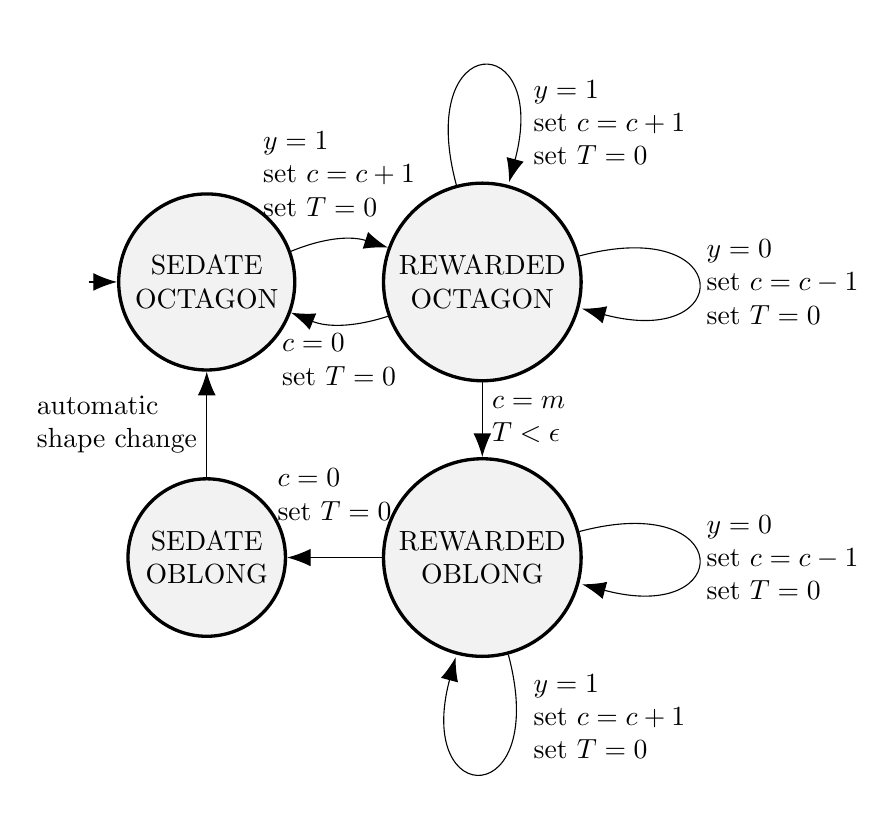
\begin{tikzpicture}[-{Latex[length=3mm]},
roundnode/.style={circle, draw=black!120, fill=black!5, very thick, minimum size=18mm}]
%Nodes
\node[roundnode,align=center] (start) at (6.5,10) {SEDATE \\ OCTAGON};
\node[roundnode,align=center] (social) at (10,10) {REWARDED \\ OCTAGON};
\node[roundnode,align=center] (tired) at (10, 6.5) {REWARDED \\ OBLONG};
\node[roundnode,align=center] (lonely) at (6.5, 6.5) {SEDATE \\ OBLONG};

\path (start) edge[bend left=20] node[above, yshift=5pt, align=left] {$y = 1$\\set $c=c+1$\\set $T=0$} (social);
\path (social) edge[bend left=20] node[below, align=left] {$c = 0$\\set $T=0$} (start);
\path (social) edge node[right, align=left] {$c=m$\\$T<\epsilon$} (tired);

\path (5, 10) edge node[above, align=left]  {} (start);
\path[every loop/.append style=-{Latex[length=3mm]}] (social) edge [loop above] node[anchor=west, xshift=15pt, yshift=-20pt, align=left] {$y = 1$\\set $c=c+1$\\set $T=0$} (social);
\path[every loop/.append style=-{Latex[length=3mm]}] (social) edge [loop right] node[align=left] {$y = 0$\\set $c=c-1$\\set $T=0$} (social);
\path[every loop/.append style=-{Latex[length=3mm]}] (tired) edge [loop below] node[anchor=west, xshift=15pt, yshift=20pt, align=left] {$y = 1$\\set $c=c+1$\\set $T=0$} (tired);
\path[every loop/.append style=-{Latex[length=3mm]}] (tired) edge [loop right] node[align=left] {$y = 0$\\set $c=c-1$\\set $T=0$} (tired);

\path (tired) edge node[above, yshift=10pt, align=left] {$c=0$\\set $T=0$} (lonely);
\path (lonely) edge node[left, align=left] {automatic \\shape change} (start);
\end{tikzpicture}
\caption{An automata representation of the on-board algorithm for distributed density estimation and reactive shape-change. The algorithm requires as input the value $m$ representing the maximum counter value on each bot and the morph threshold $\epsilon$.}
\label{fig:algo}
\end{figure}

Instead of agents making a decision when they reach a specific physical location as in the foraging context in \cite{pavlic2021quorum}, agents change shape in response to changing estimated encounter rate. We expect that groups of oblong robots will align and aggregate for longer amounts of time due to geometric frustration of their random movements, while convex octagonal robots are more likely to move away from each other after a collision.


The use of a maximum value for the counter creates an additional tunable parameter. This parameter gives a small level of control over a group of robots. With a larger maximum counter value, a higher number of neighbor encounters are needed to trigger a shape-change, increasing the dwell time in the sedate shape. With a smaller maximum counter value, the robots will switch between the two shapes more frequently since they need less stimulation. Depending on the environment the group is operating in, frequent changes in shapes could be more desirable than infrequent changes, or vice versa. Further analysis of the effect of geometry on collective state is given in Section \ref{sec:analysis}.


\begin{algorithm}
\label{alg:one}
\caption{Pseudo-code of the control law operating on board each robot. The timer $T$ is assumed to be continuously incrementing.}
\KwIn{Counter value $c$, maximum value $m$, timer $T$, bot's state ($OCTAGON$ or $OBLONG$), bot's stimulation state $STIM$, binary contact sensor $y=\{0,1\}$}
\tcc{Observe new sensor event; reset timer and bot rewarded}
\If{\not $STIM$ \textbf{and} $y=1$}{
    $STIM \gets True$\;
    $T \gets 0$\;
}
\tcc{Timer is below threshold and bot is rewarded}
\ElseIf{$STIM$ \textbf{and} $T < \epsilon$ \textbf{and} $y=1$}{
    $T \gets 0$\;
    \tcc{Counter has incremented to max value; change shape}
    \If{$c == m$ \textbf{and} $OCTAGON$}{
        $OCTAGON \gets False$\;
        $OBLONG \gets True$\;
    }
    \tcc{Counter is not at max; just increment counter}
    \If{$c$ \not $m$}{
        $c \gets c+1$\;    
    }
}
\tcc{Timer reaches threshold without a sensor event; bot sedate}
\ElseIf{$T >= \epsilon$ \textbf{and} $y=0$}{ 
    $T \gets 0$\;
    $STIM \gets False$\;
    \tcc{Counter reads zero, change shape back}
    \If{$c == 0$ \textbf{and} $OBLONG$}{
        $OBLONG \gets False$\;
        $OCTAGON \gets True$\;
    }
    \tcc{Otherwise, decrement counter}
    \If{$c$ \not $0$}{
        $c \gets c-1$
    }
}
\end{algorithm}



\section{ALGORITHM ANALYSIS} \label{sec:analysis}

We performed an analytical analysis of expected shape distribution as a function of $\epsilon$, $m$, and other system parameters. This analysis extends work done in \cite{mayya2018localization} using a hard-core Poisson process model to model the spatial distribution of robot agents. Because of the significant assumptions involved in this modelling process, we also analyze our algorithm via Monte Carlo analysis of simulated system executions. Finally, we also include a demonstration of our proposed algorithmic scheme onboard a minimalist robotic platform in a laboratory setting.

In both hardware and simulation, we implemented Algorithm \ref{alg:one} and investigated the effect of the threshold parameter $\epsilon$ and the counter $m$. Since the encounter rate is directly related to local agent density, we also varied the number of agents in a fixed-size environment.

\subsection{Analytical Analysis}

\subsubsection{Dwell Time}

 Following the reasoning in \cite{pavlic2021quorum}, we model our system with the dynamics

 \begin{align}
     \dot{R} = S \lambda - R/\tau \\
     \dot{S} = R/\tau - S \lambda
 \end{align}

  where $R$ is the fraction of the population in the (Rewarded) Oblong state, $S$ is the fraction of the population in the (Rewarded or Sedate) Octagon state, $\lambda$ is the transition rate from Octagon to Oblong, and $\tau$ is the mean dwell time after which the Oblong robots become Octagonal again.
  
  In practice, $\lambda$ and $\tau$ are determined by both the timer threshold $\epsilon$ and the timer counter maximum $m$, as well as the robot density and velocity. Here, we derive analytic expressions for both of these quantities in terms of the robot system design parameters.

\begin{lemma} \label{lem:nocollide}
The probability that a robot with radius $r$ and velocity $v$ in an environment with robot density $\rho$ experiences an elapsed time between collisions greater than $\epsilon$ is given by

\begin{equation}
\Pr(t \geq \epsilon) = \exp(-\epsilon\Omega(\rho, v, r)).
\end{equation}

where $\Omega(\rho, v, r)$ is the expected number of collisions in unit time given by

\begin{equation*}
\Omega(\rho, v, r) = 2r \frac{4}{\pi} v \chi(\rho, r) \rho
\end{equation*}

with 

\begin{align*}
    \chi(\rho, r) & = \frac{2\pi r^2}{ r^2 (\pi - k)(1-e^{-\pi r^2 p})}\Bigl[1 - \frac{1-e^{-p(2\pi r^2 - kr^2)}}{(2\pi r^2 - k r^2)(1-e^{-p \pi r^2})}\Bigr], \\
    k & = 8\pi/3 - \sqrt{3}, \text{and} \\
    p & = \frac{1-e^{-\rho \pi r^2}}{\pi r^2}
\end{align*}

\end{lemma}

\begin{proof}
The result is adapted directly from Observation 2 in \cite{mayya2019closed}. We use the corrected number of encounters per unit time and do not consider a sensing radius extending beyond the robot body.
\end{proof}

From Lemma \ref{lem:nocollide}, we compute our system dwell time in the Rewarded Oblong state, $\tau$, as a function of the system design parameters. 


\begin{lemma}
The mean dwell time of the robotic system in the Oblong shape is given by

\begin{equation*}
  \tau = e^{\epsilon \Omega(\rho, v, r)}.  
\end{equation*}

\end{lemma}

\begin{proof}
Our robotic system exits the Oblong state whenever the time between collisions is longer than $\epsilon$. Since the probability of time between collisions exceeding $\epsilon$ is exponentially distributed with rate $\Omega(\rho, v, r)$, the wait time until one of the inter-arrival times of the collision events exceeds $\epsilon$ can be modelled with a geometric random variable with success probability $p$, where ``success'' is a long interarrival, such that

\begin{equation*}
P(K=k)=(1-p)^{k-1}p \text{ for $k=1,2,\dots$}
\end{equation*}

thus giving the expected dwell time before a timer ``expires`` as $\tau = E[K]=1/p=e^{\epsilon \Omega(\rho, v, r)}$. 

\end{proof}

Now that we have determined the dwell time of our system in the Oblong shape, we must determine the transition rate $\lambda$ from Octagon shape to Oblong.


  \begin{lemma}
Let $\lambda(m, r, v, \rho, \epsilon)$ be the probability of a single robot experiencing $m$ collisions with other robots, such that the time interval between any two consecutive collisions is less than $\epsilon$. This is the necessary condition for shape-change in our system. All robots are assumed to have radius $r$, velocity $v$, and are distributed in the environment according to a Poisson hard-core point process with intensity (robots per unit area) $\rho$.
  
The probability of this event, triggering the transition from Rewarded Octagon state to Rewarded Oblong, is given by

\begin{equation*}
\Pr(N) = (1 - \Pr(t \geq \epsilon))^m
\end{equation*}

where $\Pr( t \geq \epsilon)$ is given in Lemma \ref{lem:nocollide}.
  \end{lemma}

\begin{proof}
    By our mean-field assumption, we assume that collision events are independent and our system is memoryless. This allows us to treat our $n$ sequential collision events as independent sequential events, yielding the result. Also because of our mean-field assumption, we can treat this probability as our system transition rate $\lambda$.
\end{proof}



% \subsubsection{Equilibrium half-saturation point}
%  The half-saturation point of this system at equilibrium occurs when $\dot{R} = \dot{S} = 0$ and $R = S = 1/2$. This is the system state where agents are equally likely to be in either morphology, and the population dynamics have stabilized. From \cite{pavlic2021quorum} we note this point occurs when

% \begin{equation}
% \lambda^* = \frac{\ln(2)}{\tau}
% \end{equation}

% where $\lambda^*$ is the critical transition rate for half-saturation, and $\tau$ is the mean dwell time of our system in the stimulated oblong state.

% This relation implies that given a fixed encounter rate, we may control the distribution of agents in each shape (the ``shape distribution'') by varying $\tau$. Likewise, we may expect that as the encounter rate changes, the shape distribution will also change.



\subsection{Monte Carlo Simulations}  \label{sec:sim}

% \subsubsection{MIPS index normalization} The MIPS index is an averaged index of variance over multiple window sizes and requires minimal per-system tuning; for the details of its computation see ~\cite{hao2022controlling}. To normalize the index, the index will be maximized when all agents are aggregated in a single tight cluster, and will be minimized when the agents are uniformly distributed. Due to the difficulty of finding the globally optimal extremal configurations, we used global attraction to the center of the arena to implement the maximum-aggregation case, and placed agents with equidistant repel forces to one another for the minimum-aggregation case. With this approach we are likely over-estimating the minimum MIPS index, and our MIPS index plots are not perfectly normalized between zero and one.


\subsubsection{Robot Model}

For our simulated agents, we adopt an Active Brownian motion model from \cite{shaebani2020computational} leading to the dynamical system

\vspace{-1em}

\begin{align} \label{eq:eom1}
\dot{x} & = D \left( F_{active}(\theta) + \xi(t)\right) \\
\dot{\theta} & = D_r \xi_r(t) \label{eq:eom2}
\end{align}

%\vspace{-1em}

where $x$ is the position of the robot, $\theta$ its orientation, $D$ and $D_r$ are linear and rotational diffusion constants, $F_{active}$ is the self-propulsion force (aligned with robot orientation), and $\xi$ and $\xi_r$ are uncorrelated random force and torque. We assume our agents move in $\mathbb{R}^2$, and we assume $\xi$ and $\xi_r$ are Gaussian and von Mises distributions, respectively, each with a mean of zero.

The main purpose of this model is for ease of calibration of our simulated robots to match the physics of our testbed agents. Calibration is done by determining the diffusion constants and characteristic noise timescale from tracked single bots, as described in Sec.~\ref{sec:hardware}.

\subsubsection{Simulation Implementation}

A screenshot of the simulator with 100 bots is shown in Fig.~\ref{fig:sim}. The simulator was implemented using PyMunk \cite{Blomqvist_Pymunk_2023}, a two-dimensional physics simulator. The simulation runs for 30 timesteps in between each progression of the morph to improve simulation stability, especially in cases where agents are changing shape while in contact with each other or the environment. The timestep of the simulation was chosen so that snapshots at each morph step could be rendered at 30 frames/second, so $dt = \frac{1}{900} \approx 0.001$ seconds. Larger $dt$ was found to significantly degrade simulation stability.

As this physics simulator is most stable when provided with forces on all bodies, rather than directly setting the velocity of the robots, we took the time derivative of the equations of motion (Eqs.~\ref{eq:eom1} and \ref{eq:eom2}) and thus assumed a constant force, proportional to $D$, along the heading $\theta$. In practice, micro/nano-scale active particles quickly achieve a maximum speed when propelling and are effectively non-inertial. For the simulation, we implemented a controller for each agent to quickly achieve and maintain a constant velocity.

To simulate system noise, we apply a random reorientation force at uncorrelated random times. During hardware characterization we found an expected reorientation timescale of $\tau=1.2$ seconds, so we would expect a reorientation every $\epsilon = 1.2/dt = 1080$ timesteps. At each timestep, we sample a uniform random variable in $[0,1]$ and check if it is less than $1/\epsilon$. If so, we sample a vector uniformly from the unit circle, scale by the linear diffusion constant $D$, and use this quantity as our new constant propelling force. With this method, we respect the uncorrelated aspects of rotational and linear diffusion in the system.% The resulting physics are essentially the run-and-tumble model of active particles, rather than the more slowly reorienting original Active Brownian particle model. While these two motion strategies have very similar physical properties in bulk and confinement at large scales, they do exhibit some interesting differences at small scales \cite{khatami2016active}, a possible subject of future study with this platform.

The simulator allows for custom environments and control of agent density, speed and mass. The simulation code is available upon request.

% \subsubsection{Effect of Shape Change on Encounter Rate}

% To validate our assumption that collision rate is largely independent of robot shape, we varied the number of bots from five to forty, and the threshold $\epsilon$ from five to forty seconds. For each combination, we simulated two minutes of collective behavior, and performed five simulations with random initial conditions. The encounter rate statistics for each combination are shown in Fig.~\ref{fig:collrate}. As expected, the encounter rate increases approximately linearly with agent density and has no apparent dependence on the threshold $\epsilon$. This verifies that changing the robot shape does not significantly violate the ``memoryless'' assumption we make of our system.

 
% \begin{figure}
% \centering
% 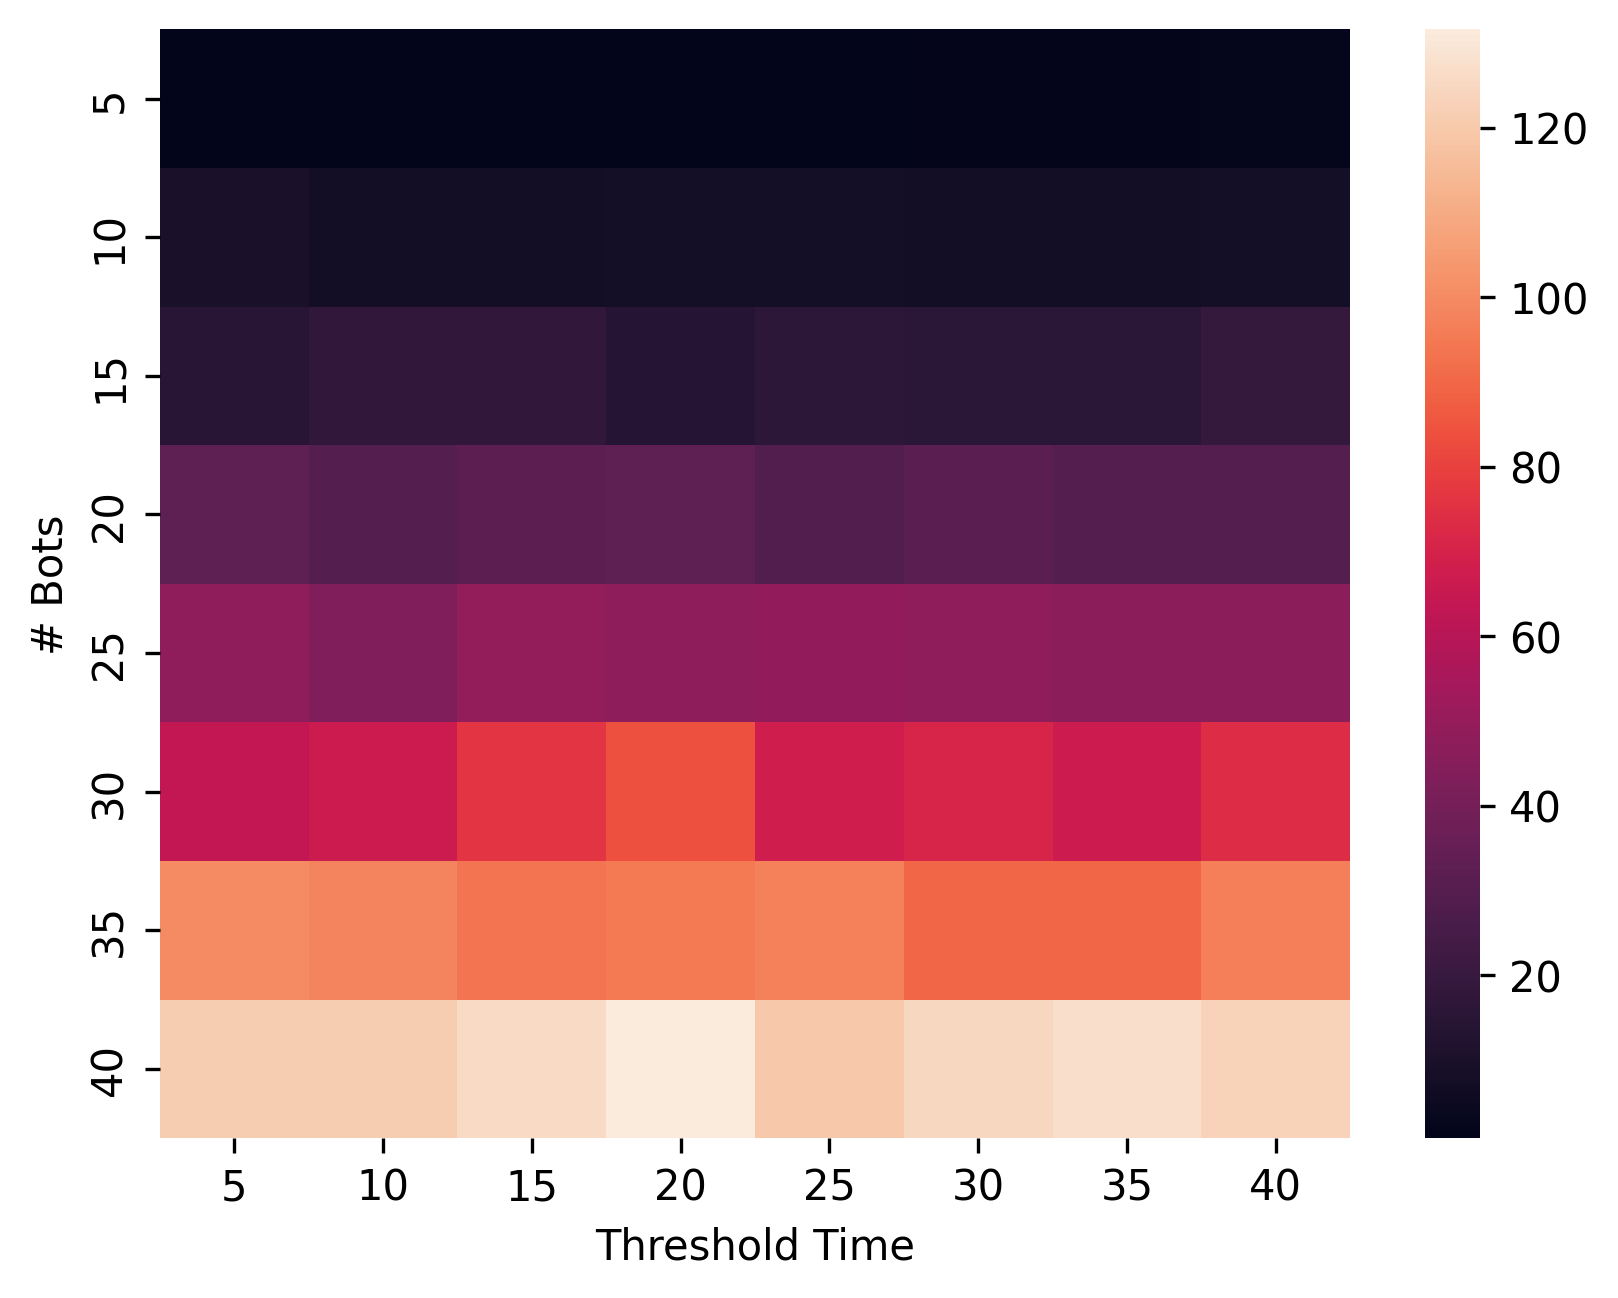
\includegraphics[width=0.4\linewidth]{figs/collision_plot.png}
% 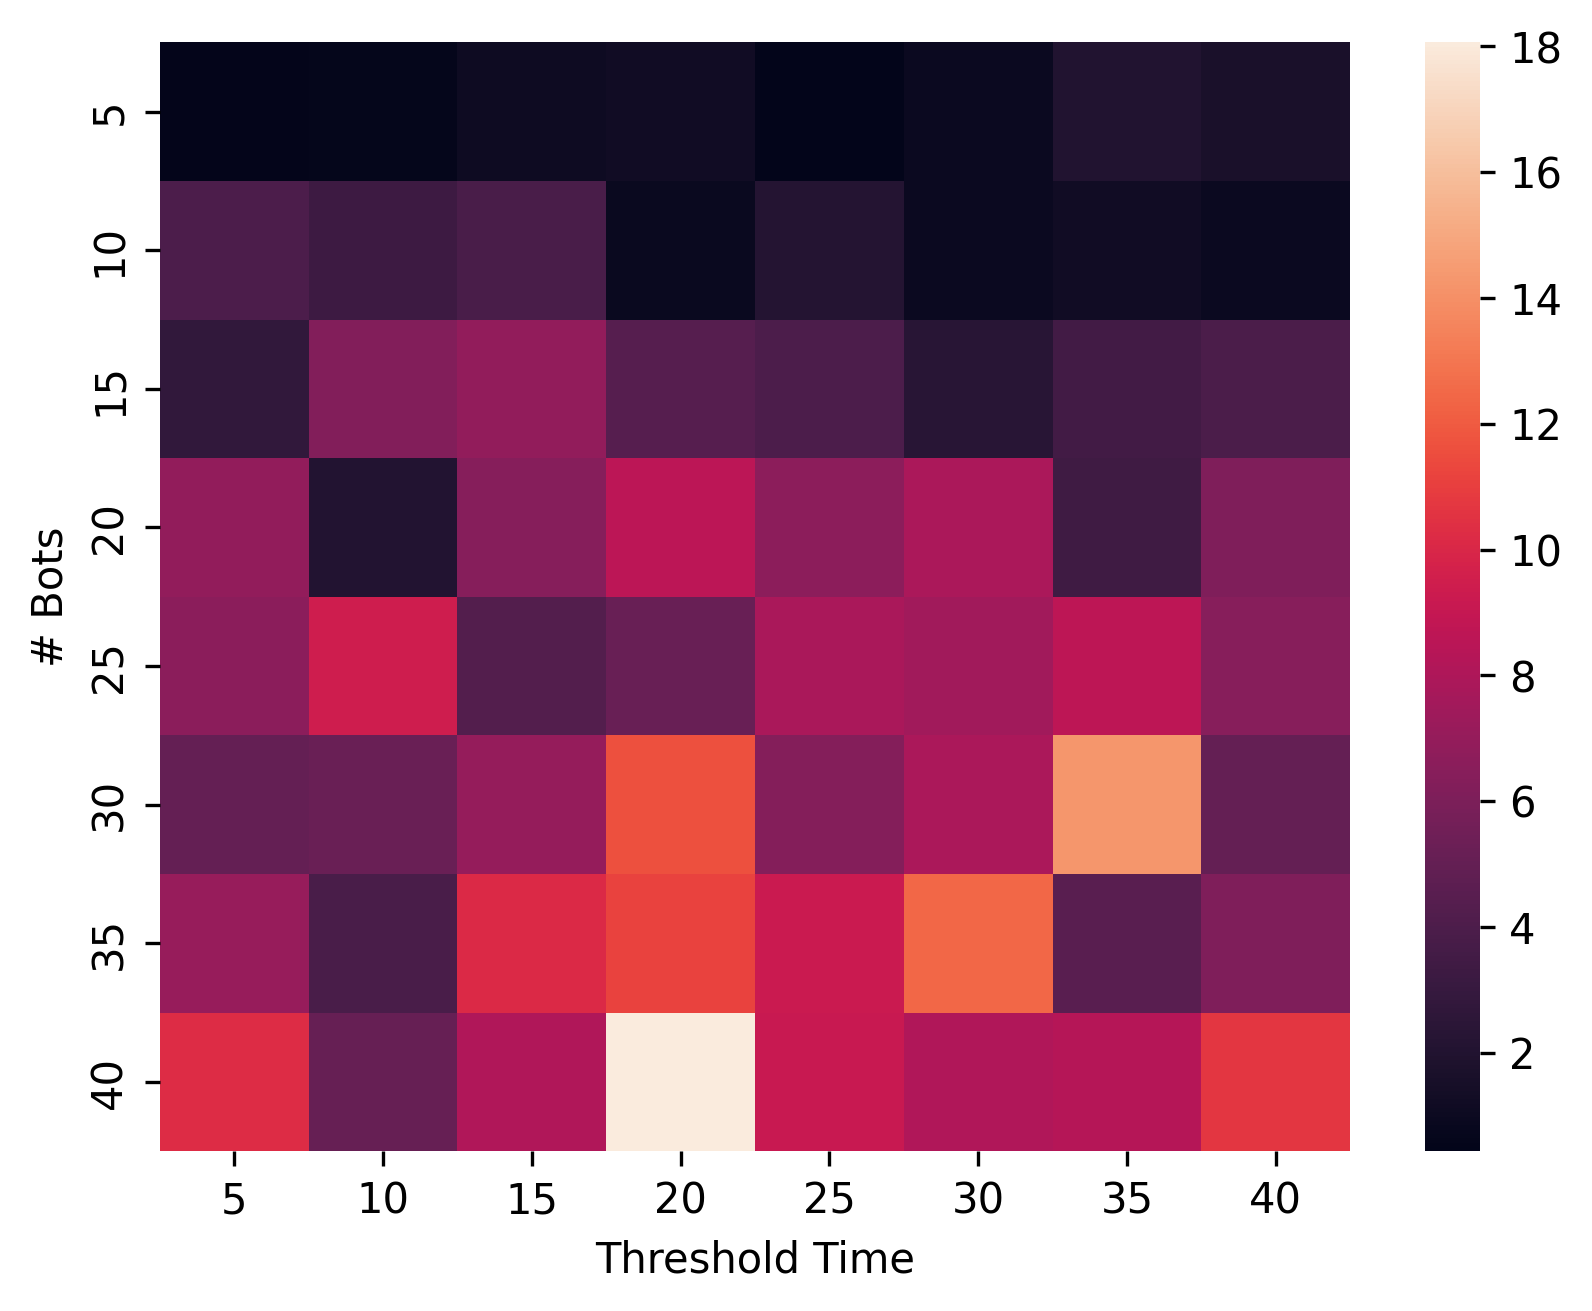
\includegraphics[width=0.4\linewidth]{figs/collision_plot_std.png}
%     \caption{(Left) Mean collision rate in simulation, in collisions per second. (Right) Standard deviation of collision rate.}
%     \label{fig:collrate}
% \end{figure}



\subsubsection{Arena Design} At the time of experimentation, we had six functional robots, and chose an arena size that facilitated a reasonable encounter rate.

 As derived in \cite{mayya2019closed}, if we model agents as hard circles with radius $r$ traveling at velocity $v$, the encounter rate $\lambda$ is expressed as

 \begin{equation}
\lambda = 4 r (4/\pi) v \rho
 \end{equation}

 where $\rho$ is the agent density per unit area.

 With this relation, we tuned the size of our arena to produce an agent density $\rho$ that will lead to a desired critical encounter rate $\lambda^*$. Our hardware experiments are done with six robots of radius $w=0.09$ meters, From the single-bot measurements described in Sec.~\ref{sec:hardware}, we estimated the linear velocity (between re-orientations) to be approximately 0.02 meters per second. From preliminary experiments, we chose a desired critical encounter rate of three encounters per minute, giving $\lambda^* = 0.05$ agents/second. These parameters give us a desired area of $1.1 m^2$ for our arena. Due to ease of construction, and experiments in \cite{pavlic2021quorum} indicating that arena shape has negligible effect on density estimation, we use a 1.05m x 1.05m square arena both in simulation and in our hardware experiments.

 We acknowledge that these calculations neglect to include effects of shape-change on agent "effective area," as well as the fact that corner and boundary effects, under certain conditions, can ``trap'' active Brownian agents. The corner and boundary effects in particular had a larger than anticipated effect at low agent numbers, and future experiments will include larger agent numbers and a smoother arena shape. The hardware design and experiments are presented here as a proof-of-concept open design for the robotics community.

\subsubsection{Effect of Threshold} In the first system behavior analysis, we hold the number of agents constant while varying $\epsilon$, the mean dwell time in the rewarded state. Fig.~\ref{fig:varythresh} demonstrates the system dynamics with $N=20$ bots. We examine both the time evolution of the populations of each morphology, and the MIPS index. While there are some intriguing periodic dynamics that appear to be present in the data, space prohibits a thorough analysis and we leave the fluctuation dynamics to a future work. For now, this analysis serves to show that given a constant density of robots, the collective shape allocation is effectively robust to the threshold $\epsilon$. However, the MIPS index appears to show a larger spread in values, though not to a point that is statistically significant (as computed by a standard t-test on the mean values at the end of the experiment). Further study is needed to understand the effect of this algorithmic approach to shape allocation and collective aggregation dynamics; while the macroscopic measures shown here are quite similar, the local interaction dynamics are still sensitive to $\epsilon$, as can be seen in the supplementary video.


\begin{figure}
\centering
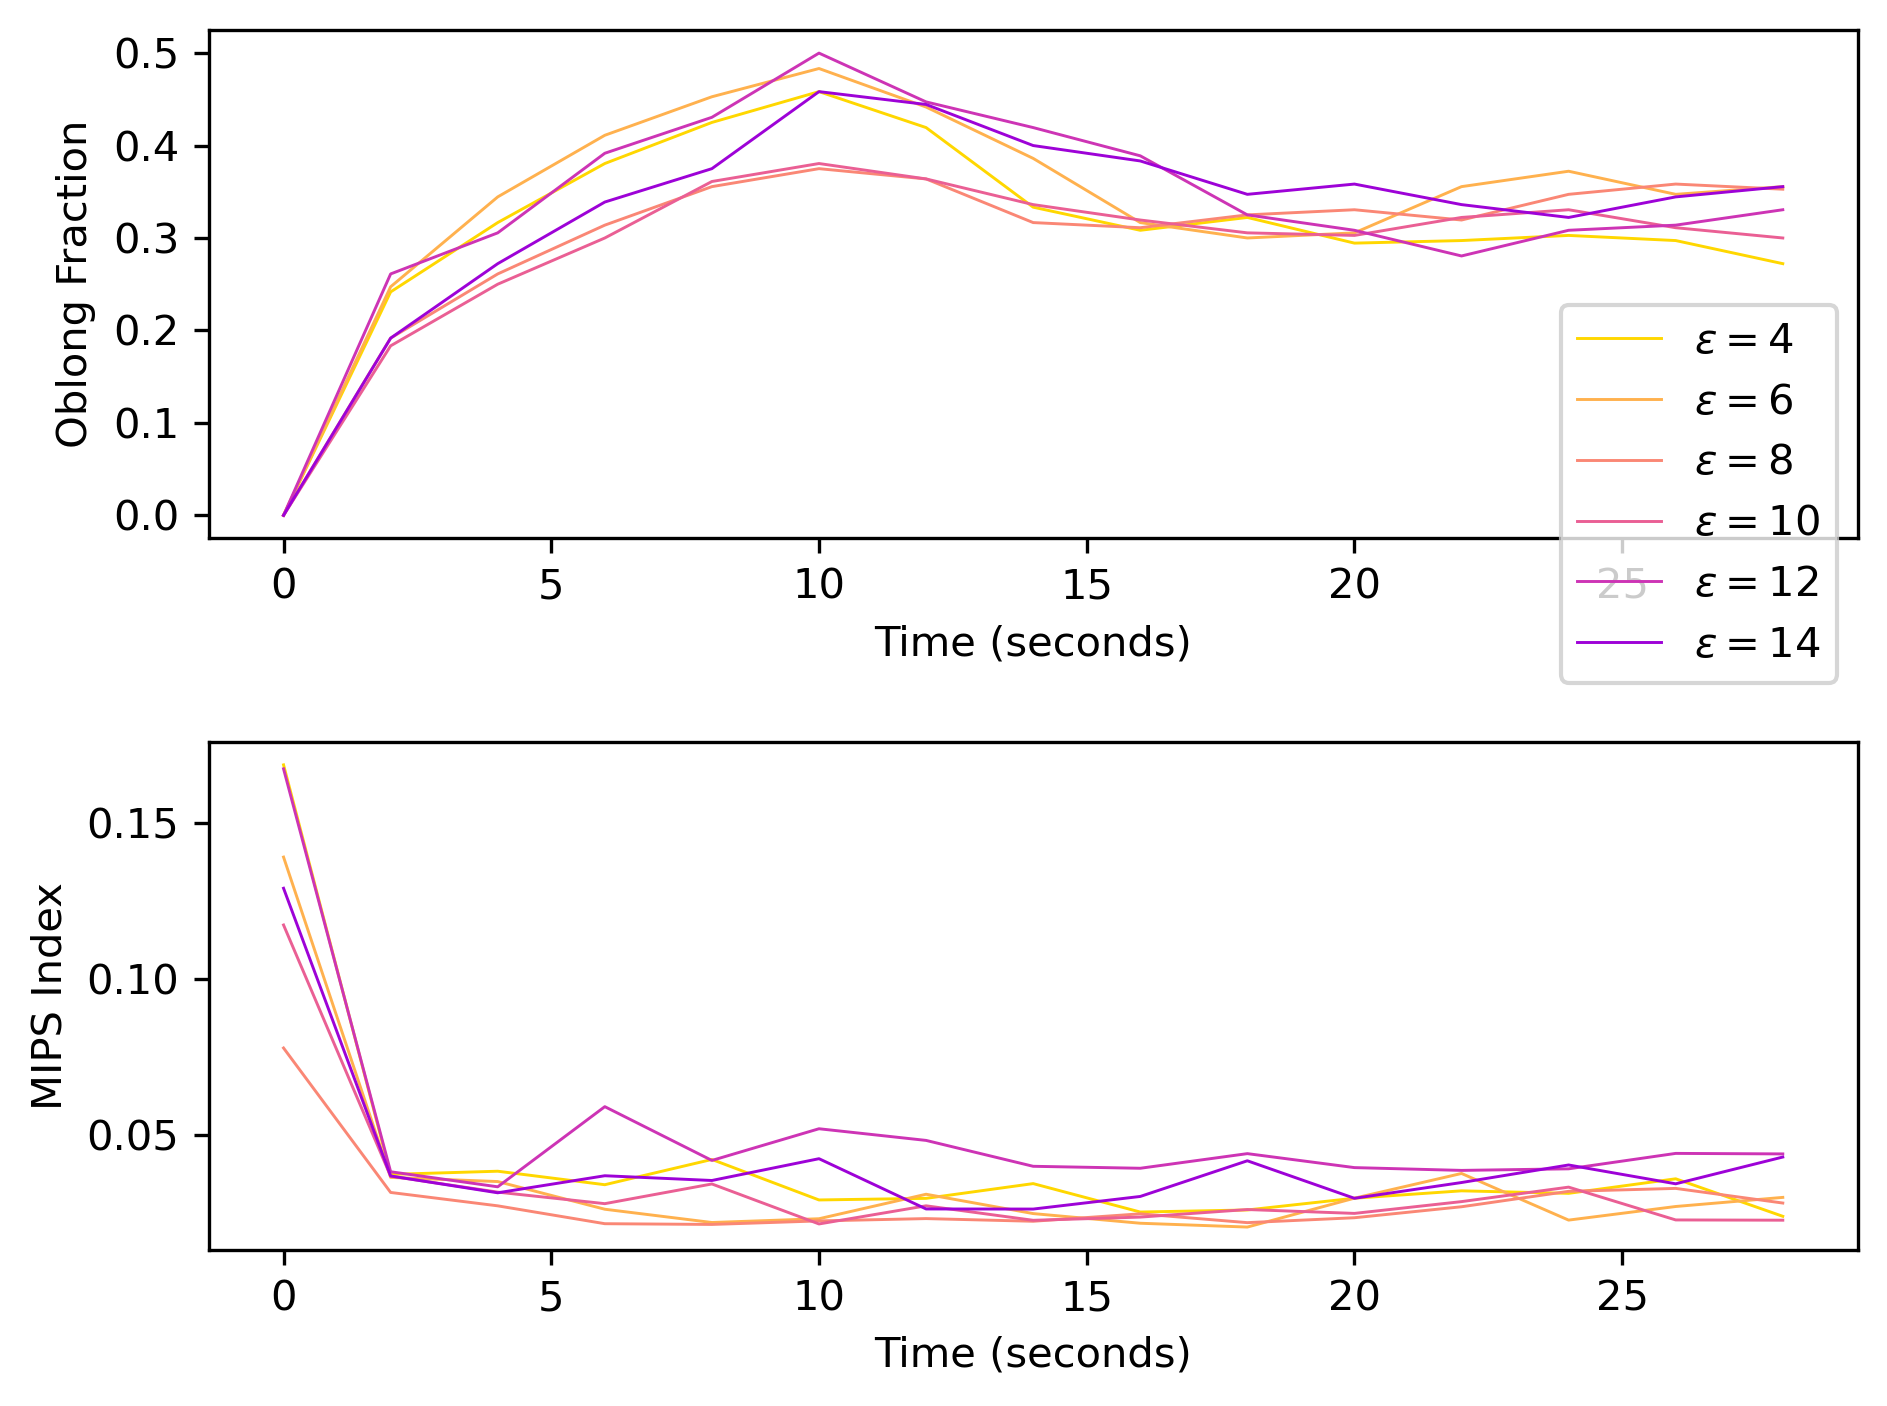
\includegraphics[width=0.8\linewidth]{figs/fracs_thresh_plot.png}
    \caption{The fraction of the collective in an oblong state, using $N = 20$ bots, and varying $\epsilon$ to examine the system sensitivity to varying the timer threshold. Each line is the average of ten trials with robots initialized in the center of the arena.}
    \label{fig:varythresh}
\end{figure}



\subsubsection{Effect of Density} As seen in Fig.~\ref{fig:varybots}, the equilibrium distribution of shapes, as well as the MIPS index, are clearly affected by the local density when $\epsilon$ is held constant. As expected, the MIPS index is roughly proportional to density, though the spread in the MIPS index is smaller than expected. The equilibrium index of shapes shows more octagonal entities, which tend to form more aggregations, mitigating the effect on the MIPS index. This is an exciting result: the robotic collective can sense and therefore adapt to changes in collective density.


\begin{figure}
\centering
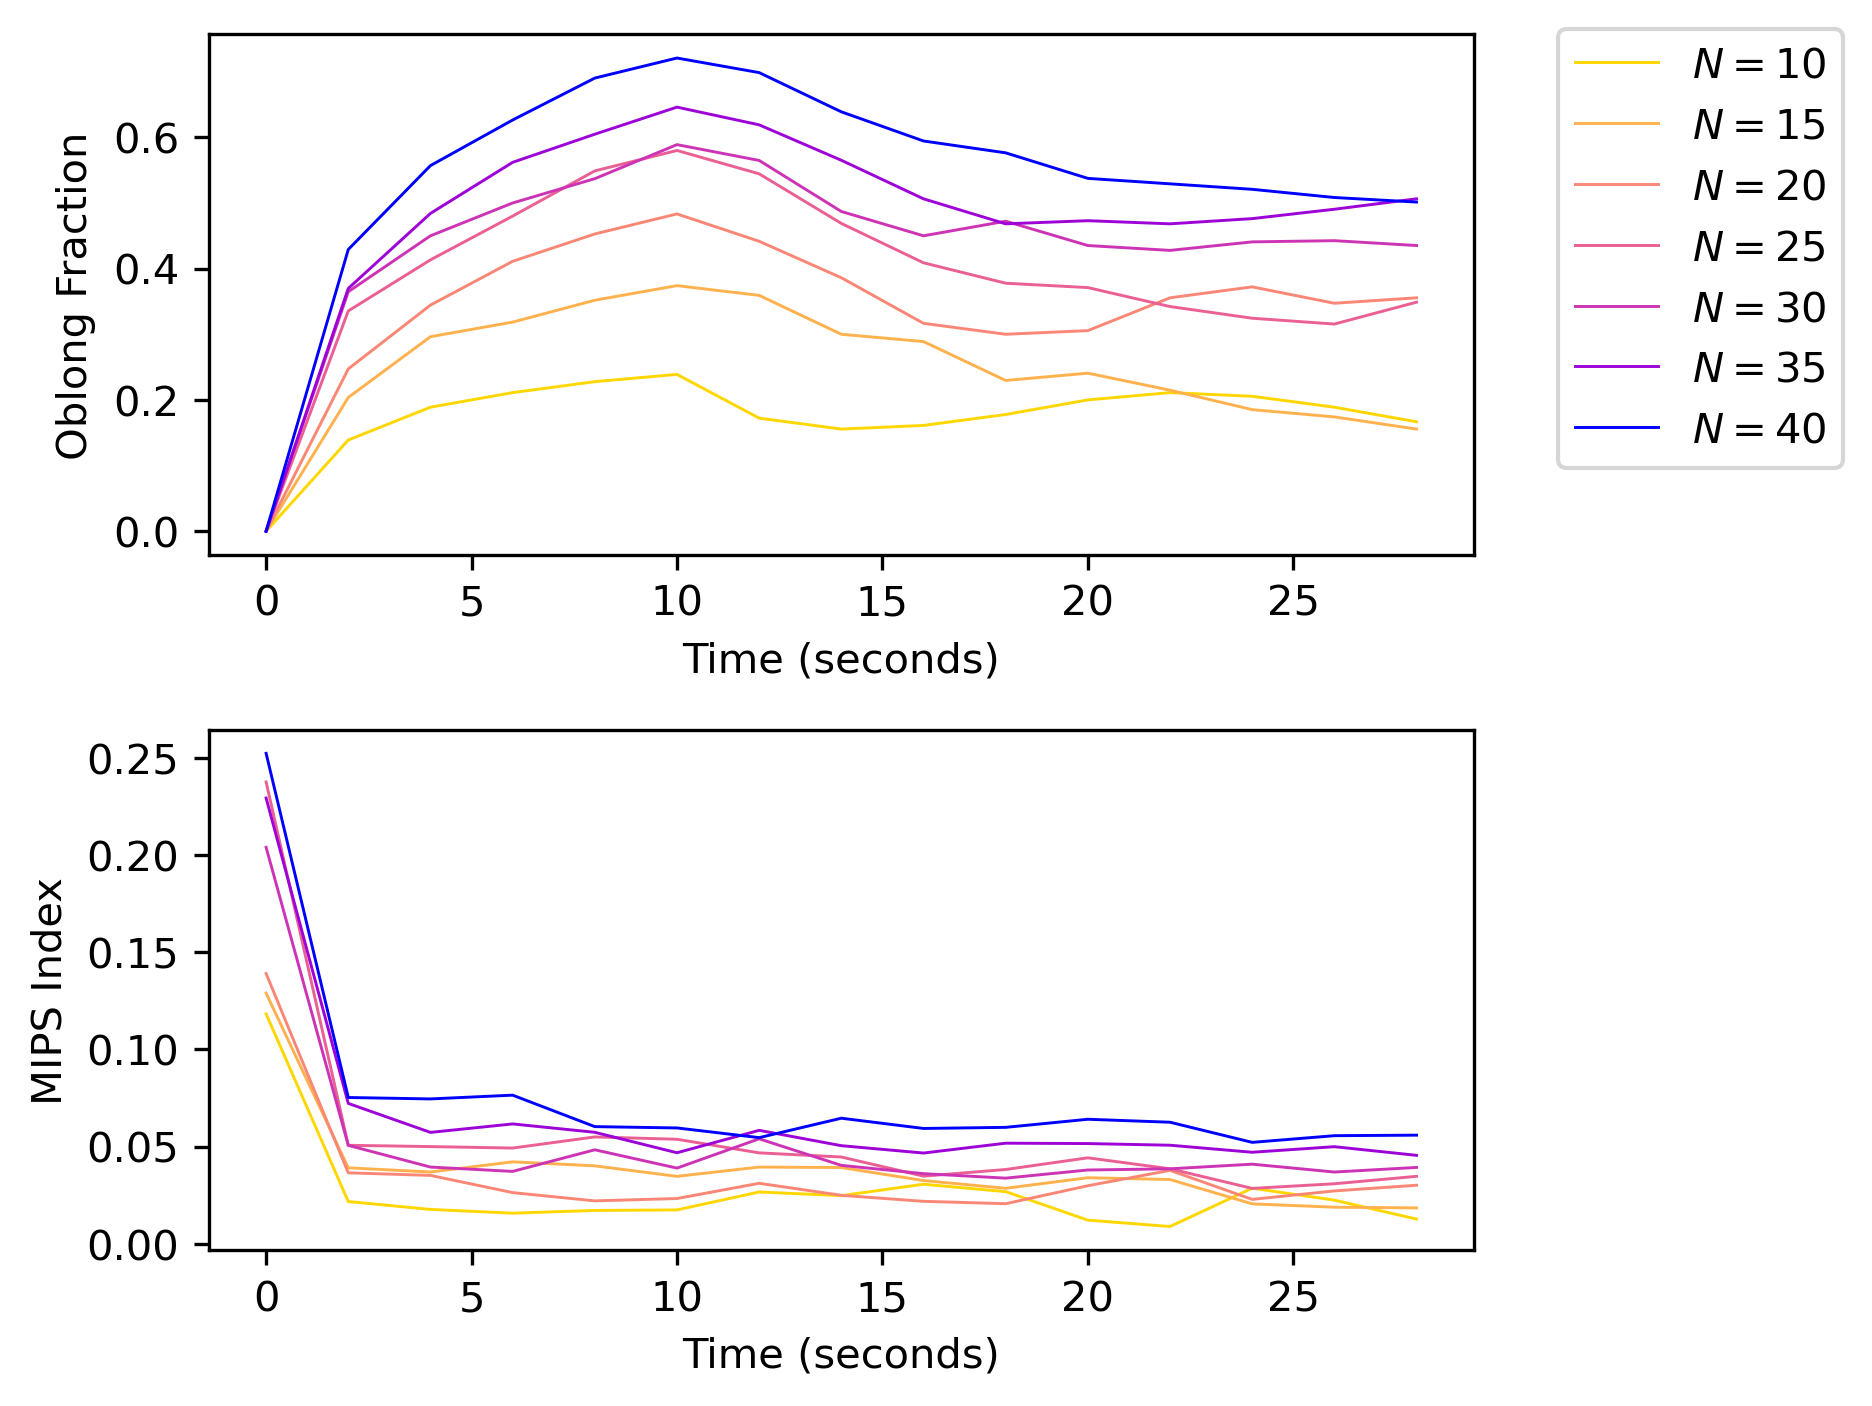
\includegraphics[width=0.8\linewidth]{figs/fracs_bots_plot.png}
    \caption{(Top) The fraction of the collective in an oblong state, using $\epsilon = 6$, and varying agent number $N$ in a fixed-size square arena to examine the effect of varying density. Each line is the average of ten trials with robots initialized in the center of the arena.}
    \label{fig:varybots}
\end{figure}


\subsubsection{Effect of Maximum Counter Value} Holding all other parameters constant ($\epsilon = 2$ and $N=100$), we investigated the effect of varying the system design parameter $m$ (the maximum counter value). In Fig.~\ref{fig:varym} we see that for small $m$, the system quickly converges to the same equilibrium state. However, as $m$ increases, the probability of the counter reaching its maximum value is $p^m$, where $p$ is the probability of a single timer being triggered by a collision before $\epsilon$ time elapses. This result implies that even in very dense environments, using a high $m$ (or requiring a high count of consecutive inter-arrival times $<\epsilon$) can serve as a method of avoiding overshoot of the target shape distribution.



\begin{figure}
\centering
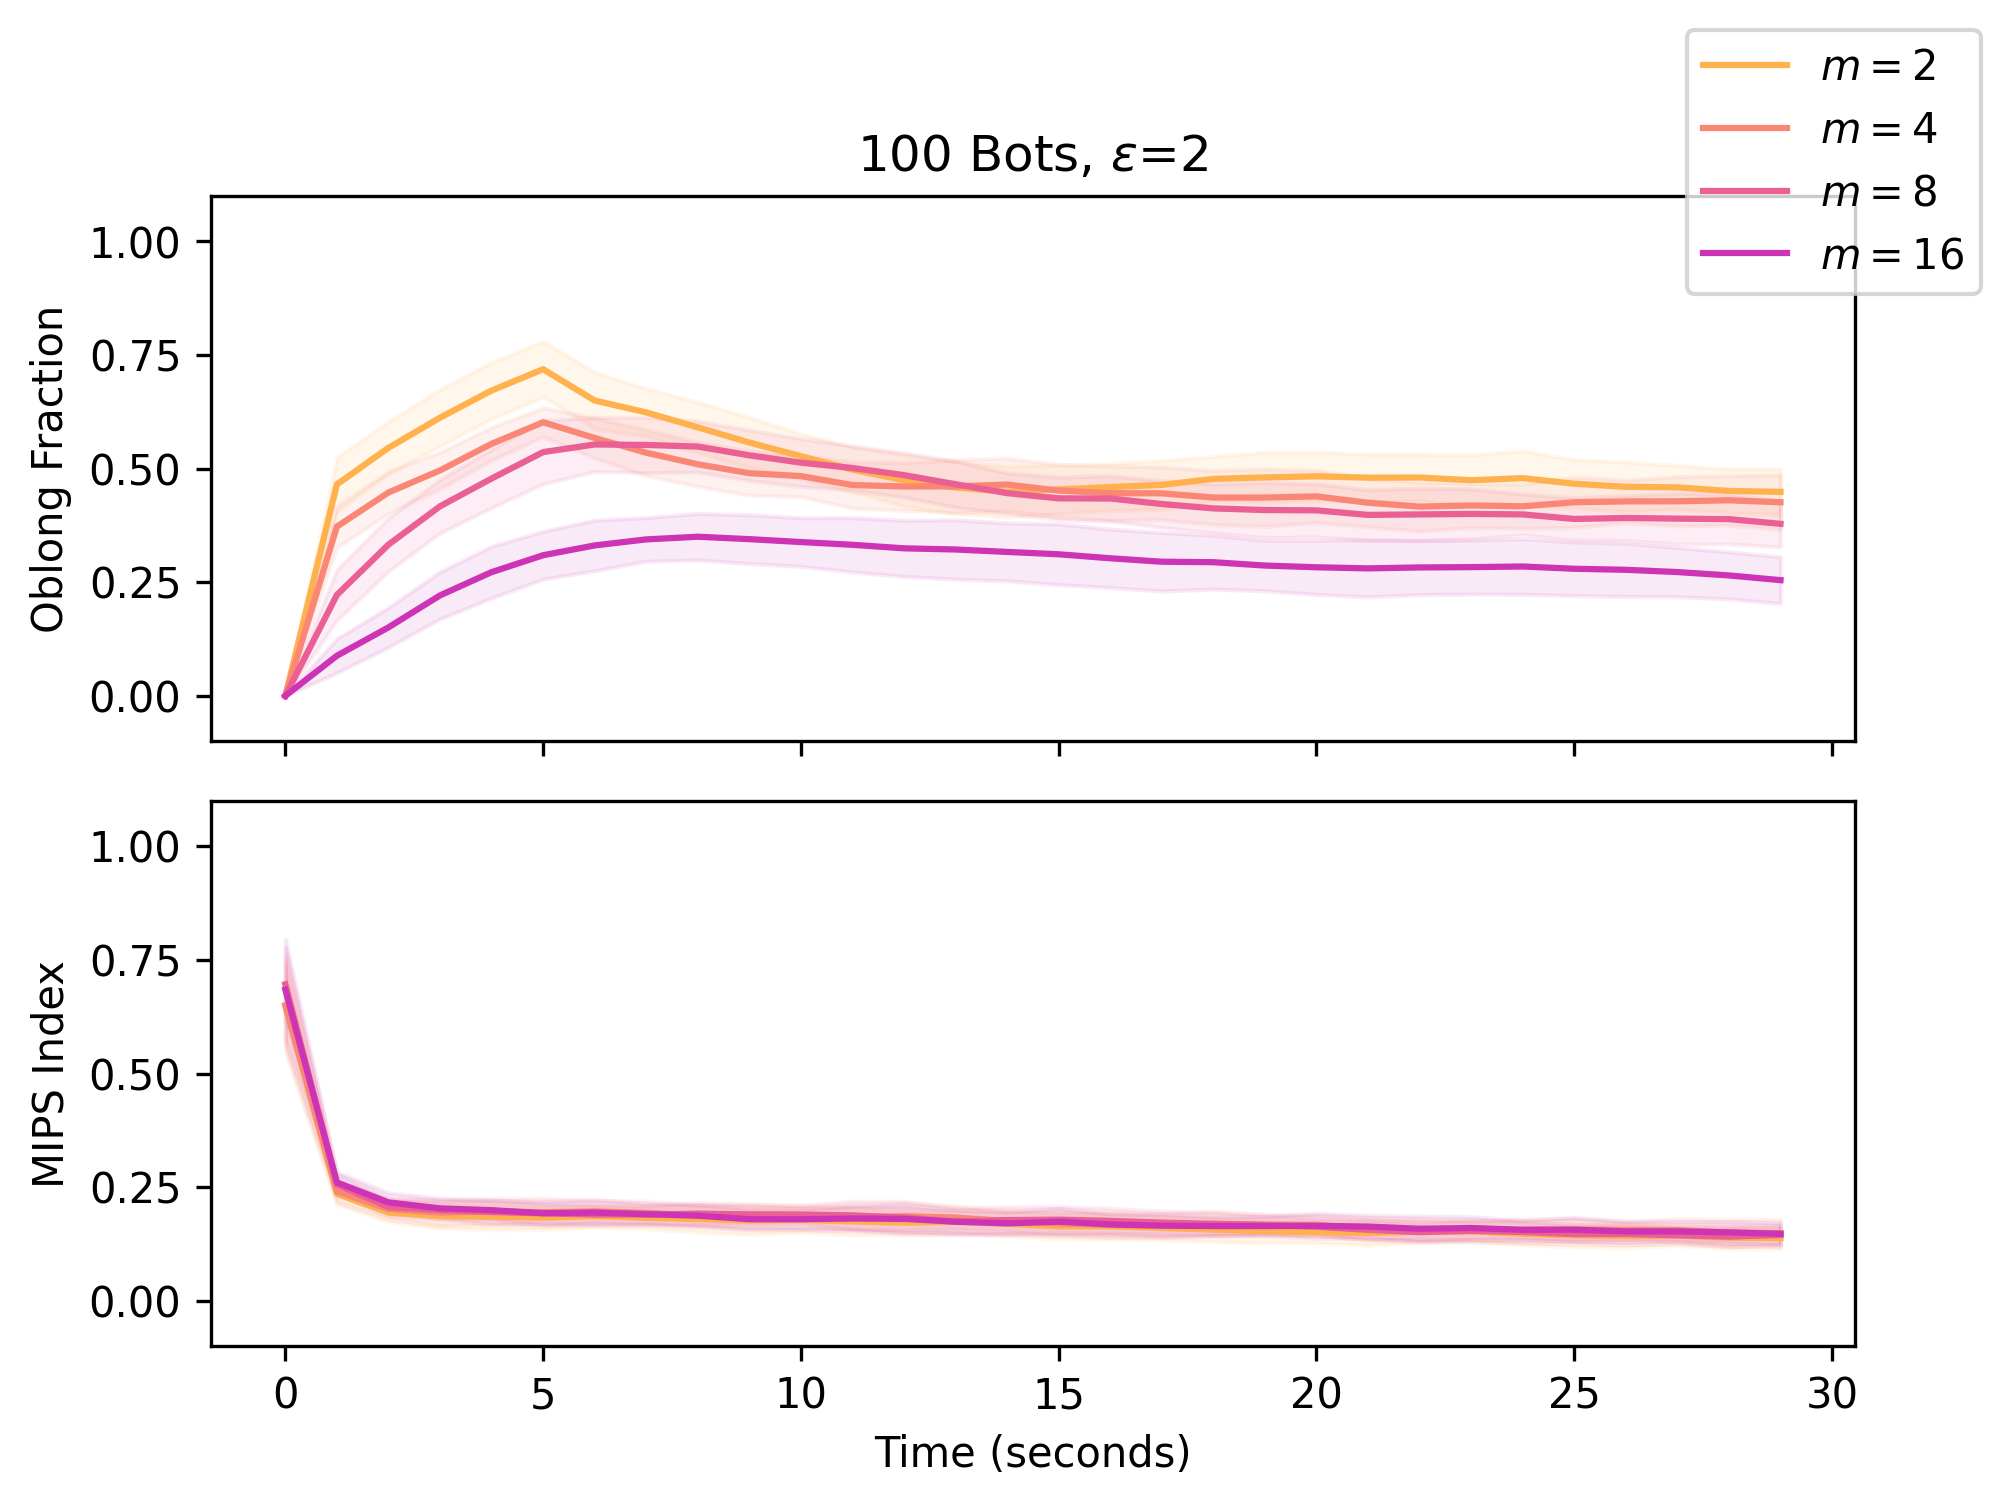
\includegraphics[width=0.7\linewidth]{figs/timer_comparison.png}
    \caption{(Top) The fraction of the collective in oblong state, using $N = 100$ bots, and varying $m$, keeping all other parameters constant. Each line is the average of thirty trials, with the shaded region indicating $\pm \sigma$ where $\sigma$ is one standard deviation over the trials.}
    \label{fig:varym}
\end{figure}


\subsection{Hardware Platform} \label{sec:hardware}


Our robots are designed as ``hubs'' on an off-the-shelf wild body, in this case a toy ball for pets driven by an internal motor with an off-center counterweight\footnote{The original manufacturers are no longer distributing the Weazel Ball used in prior studies. Many variations can be found using search keywords ``interactive self rotating cat ball'', and the particular platform used here is from manufacturer YOFUN at \url{https://www.amazon.com/YOFUN-Smart-Interactive-Cat-Build/dp/B07SYYRCYV}.}. The hub consists of a cage enclosing the propelling ball, above which are two four-link arms supporting a paper ``skirt'', as well as mounts for a PCB, a battery and two servo motors. AprilTags \cite{wang2016iros} enable motion tracking. Due to limited power of the propelling ball, we minimized the mass of the hub, totaling 23 grams. The hub is 3D-printed with PLA and PETG materials, and assembled with glue and a folded paper skirt (the \emph{water bomb} base fold in origami). The skirt extends beyond the propelling ball, so steric interactions between agents will be governed by the geometry of the paper. Our design can transform between three shapes (symmetric convex octagon, oblong, and nonconvex star) in any order. For our hardware design, we use the symmetric convex and nonconvex star shapes. For our simulation design, we use convex and oblong. Limitations in available servo motors prevented systematic testing of the oblong shape in hardware experiments. See Fig.~\ref{fig:botpics} for a photographic view of the robotic agents.

Each PCB contains an ATmega328 microprocessor and eight infrared (IR) emitter/receiver pairs equally spaced around the perimeter of the PCB. The receiver was placed underneath the PCB to shield from ambient light. We used these IR sensors to emulate an event-triggered collision sensor by programming the robot to only react when a sensor first detects a neighboring signal after a period of no IR detections.  The PCB drives two FH-1083 servos for controlling the two pairs of four-bar-linkage arms. The PCB is powered by a 3.7V 150mAh Li-Po battery. Each robot has a battery life of approximately 15 minutes when frequently actuating and sensing.

The robot arena was constructed from a single medium-density fibreboard (MDF) and was leveled with 3D-printed shims. We constructed walls for the arena from a corrugated plastic material, which we cut below the line of sight of the IR sensors, so as to prevent reflections off the walls.

\begin{figure}
\centering
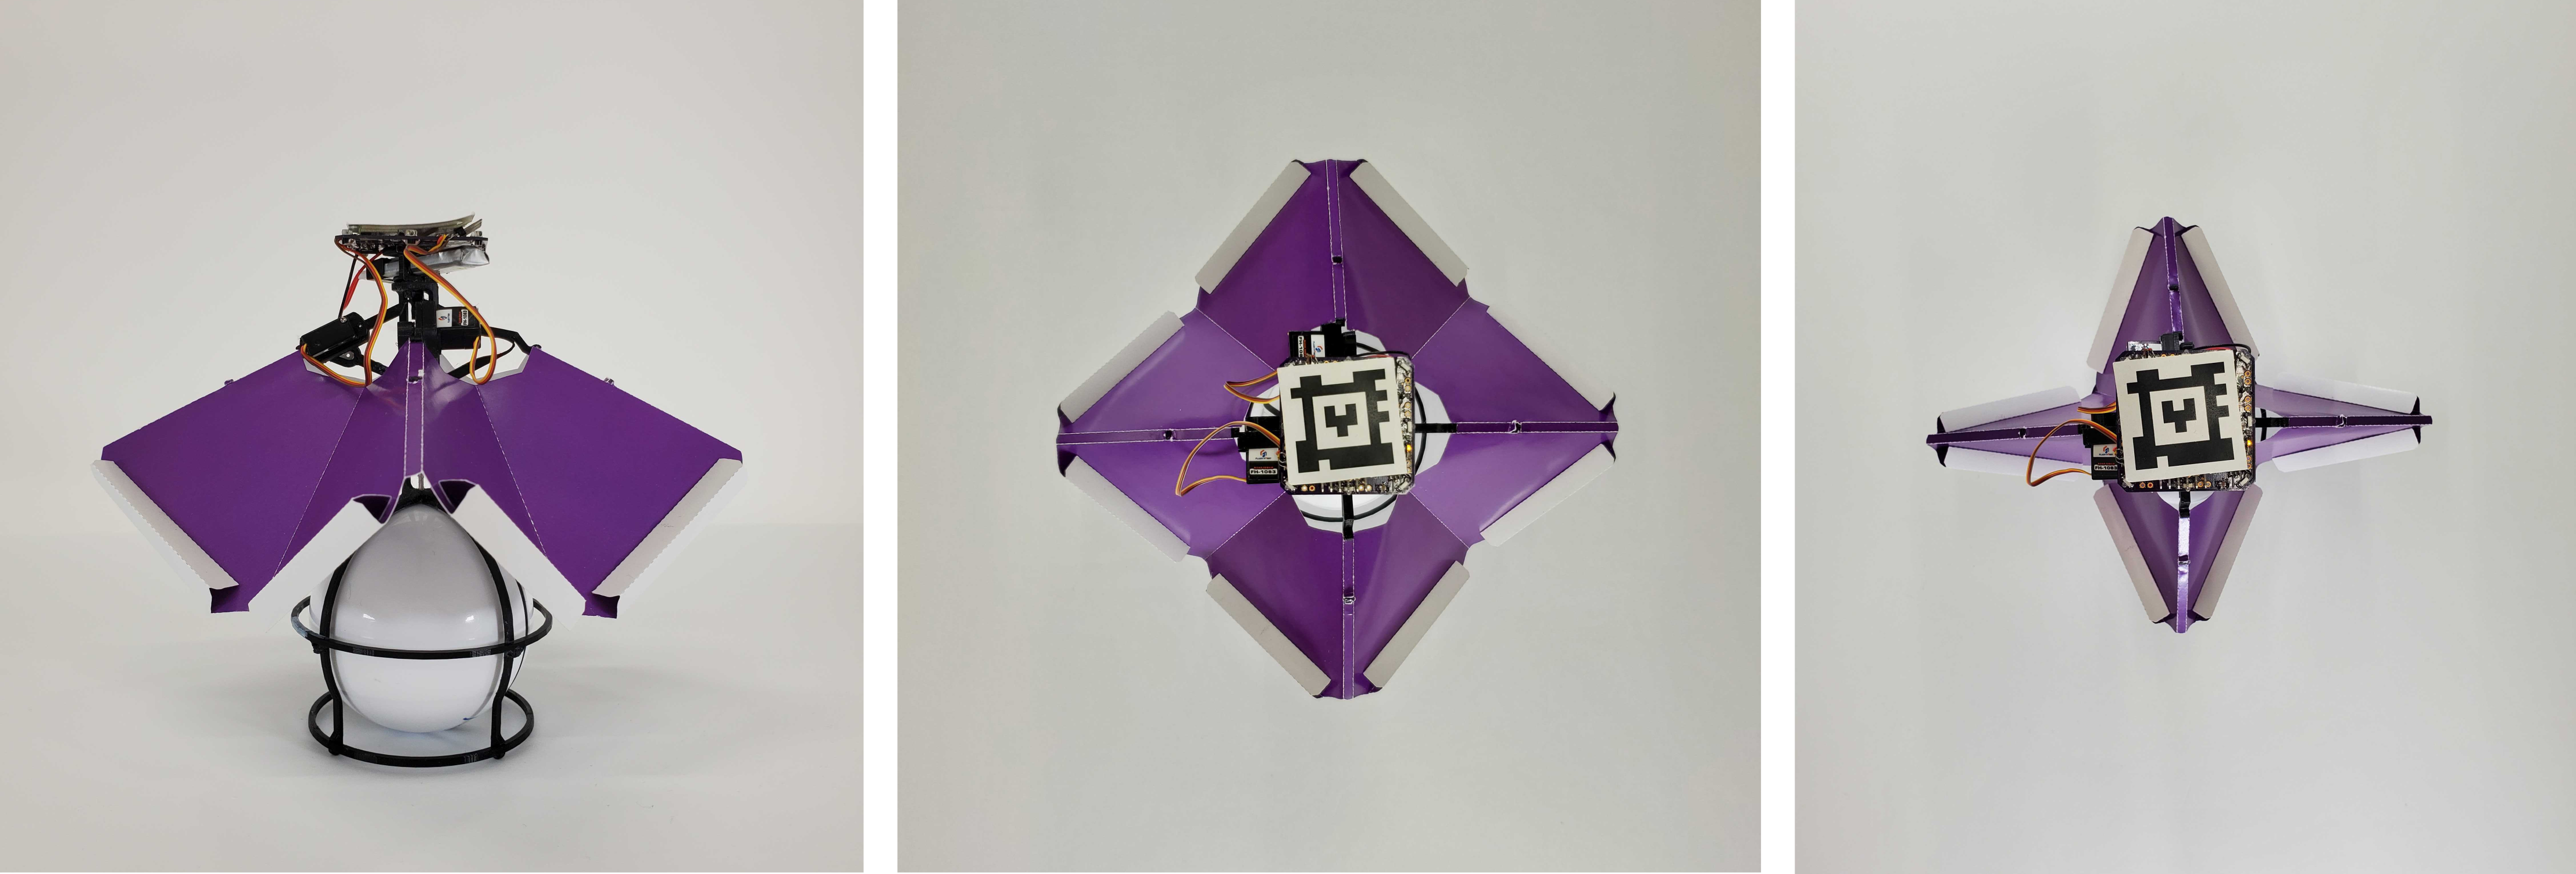
\includegraphics[height=3cm]{figs/wb-shapeshift.png}\
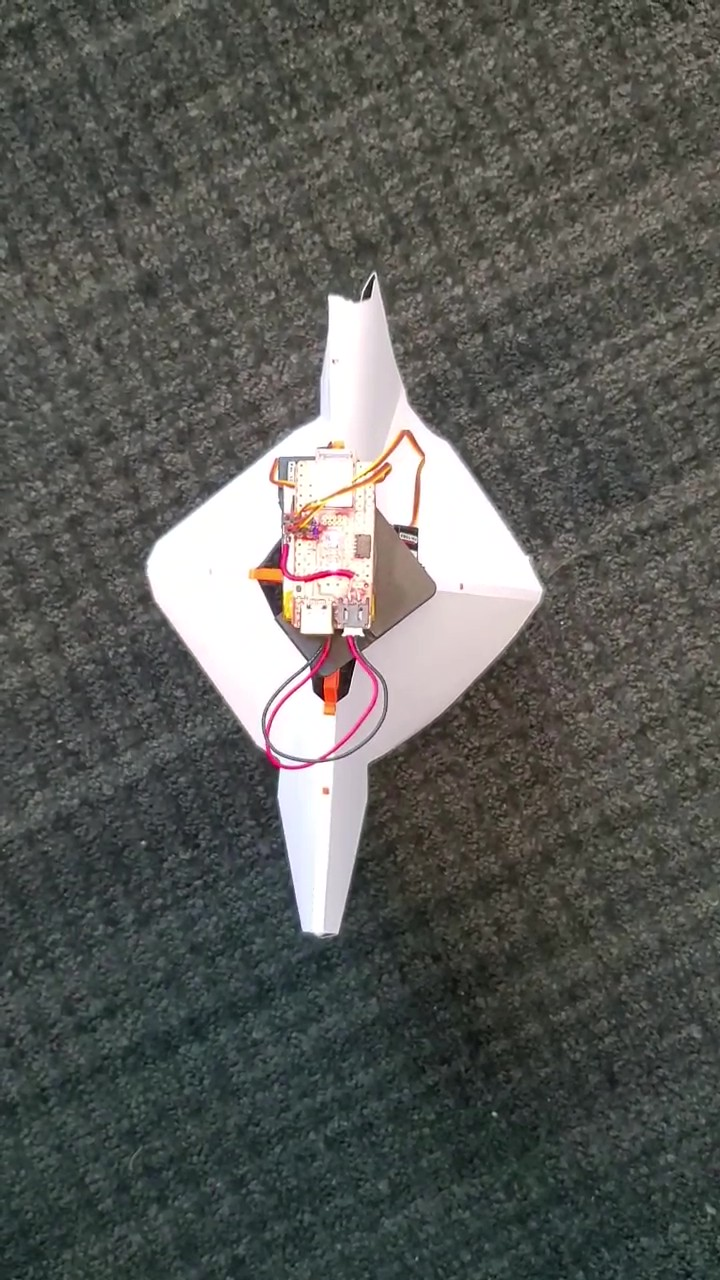
\includegraphics[height=3cm]{figs/hub_long_temp.jpg}
\caption{From left to right: our shape-shifting robotic platform from a side view, top view in convex shape, top view in nonconvex shape, and top view in elongated shape.}
\label{fig:botpics}
\end{figure}

\subsubsection{Motility Characterization} We collected thirty clips of the robot's free motion, computed the resulting mean-square-displacement (MSD) curves. The slope of the linear portion of the MSD curve is proportional to the linear diffusion constant $D$ in Eq.~\ref{eq:eom1}. Instead of separately estimating $D_R$ and the timescales of $\xi(t)$ and $\xi_R(t)$, we implemented a single random (in direction and magnitude) impulse at a timescale determined by the lag time $\tau$ for which the linear regime ends, approximately 1.2 seconds in this case. This estimation aligns with our observations of the free motion of the robots.
%During prototyping, we observed that increasing the counterweight allows the ball to push more weight, due to conservation of momentum when the ball collides with the external hub (up to the motor torque limit). Additionally, changing the counterweight results in different motility profiles for the robots. We conducted a prototyping experiment with known weights, an un-instrumented hub, and a single propelling ball in a large arena.  Based on these results, we chose a 17 gram additional counterweight to balance the objectives of maximum velocity and minimum wear to the motor and battery. 

% \begin{figure}
% \centering
% 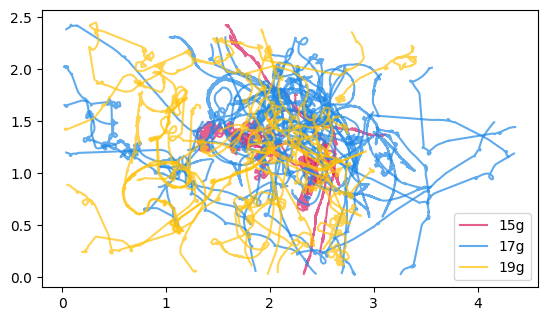
\includegraphics[width=.69\linewidth]{figs/raw_trajectories.png} 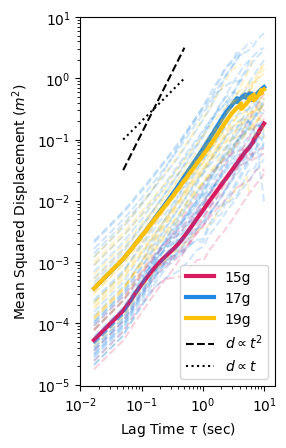
\includegraphics[width=.3\linewidth]{figs/MSD_new_design.png}
%     \caption{(Left) Raw trajectories of single bots with variable mass counterweights. (Right) Mean squared displacement curves of bots with variable mass counterweights. The mean of all trials is shown with the solid lines.}
%     \label{fig:motility}
% \end{figure}



\subsection{Hardware Demonstration}

To validate our approach with physical hardware, we programmed six robots with Algorithm~\ref{alg:one}. The bots were turned on, placed in the center of the arena, and allowed to run freely for ten minutes. Two such demonstrations were performed. As confirmed in simulation, the collective statistics are highly noisy at small $N$, but we observed frequent shape-change in response to small aggregations of robots. Clips from the demonstrations are included in our supplementary video.



\section{CONCLUSION AND FUTURE WORK}

Our findings indicate effective strategies for controlling both shape-change and extent of aggregation in collectives of uncontrollable ``wild'' robots. These strategies are perhaps most useful in micro/nano-robotic systems in crowded environments, and we plan to collaborate with micro-robotics researchers to apply these results to real-world systems. We are especially interested in combining local morphology control with uniform global control signals \cite{becker2014reconfiguring}, enabling fully decentralized collective adaptation with no direct communication between agents. This decentralized information processing is mediated entirely by the stochastic collision dynamics of the robot collective.

The off-the-shelf propelling ball used here is smaller and less powerful than the no-longer-commercially-available WeazelBall product used for previous wild bodies experiments \cite{nilles2019hardware}, which prevented us from using servo motors with the range required to achieve all three morphologies. Our minimalist design allows for effective shape-shifting between convex and non-convex shapes, but there are several weak points in the design that lead to breakdown over long-term use, limiting the analysis of hardware demonstrations. Specifically, the flexible joints of the four-arm linkages are prone to damage from repeated flexing. One advantage of our design is that the propelling body can easily be replaced within the hub. Future studies will involve propelling the hub with a small mobile robot that is programmed to emulate different types of self-propelling particles for deeper study into the links between morphology, motility, and decentralized algorithms for minimalist morphological coordination.

\begin{credits}
\subsubsection{\ackname} 
The authors gratefully acknowledge Paige Shelton, Anthony Chavez, and Danna Ma for their assistance with experiments and development of the simulator. This work was supported by NSF grant \#2042411, the Packard Fellowship for Science and Engineering, and a Cornell Engineering Learning Initiatives Award.
\end{credits}

\bibliographystyle{splncs04}
\bibliography{refs}

\end{document}
